\section{Sintonia de controladores}


\begin{frame}{Sintonia}
	\begin{block}{Introdução}
		\begin{itemize}
			\item As principais razões para a baixa performance de processos automatizados estão relacionadas ao \textbf{mau funcionamento} de válvulas, aos \textbf{sensores} e ao \textbf{ajuste incorreto} dos controladores PID.
			\item O \textbf{ajuste} (sintonia) é o trabalho de \textbf{determinar valores adequados} para \textbf{parâmetros} de um controlador, de tal modo que o processo exiba as propriedades desejadas.
			\item Apesar de \textbf{extensivos estudos} sobre esse assunto, ainda não existe um \textbf{método único} para proceder a este ajuste.
			\item Muitos controladores possuem uma função denominada \textbf{autoajuste} (self-tune) que, durante sua inicialização, a partir de um \textbf{sinal de entrada} e da \textbf{resposta obtida}, \textbf{calcula os parâmetros} do controle PID e \textbf{memoriza} os respectivos valores.
		\end{itemize}
	\end{block}
\end{frame}


\begin{frame}{Sintonia}
	\begin{block}{Introdução}
		\begin{itemize}
			\item O controlador PID possui três parâmetros de ajuste:
			\begin{enumerate}
				\item\normalsize Ganho proporcional – $ K_c $
				\item\normalsize Tempo integral – $ T_i $
				\item\normalsize Tempo derivativo – $ T_d $ 
			\end{enumerate}
			\item O projeto de um controlador nem sempre é \textbf{suficientemente completo}, e os métodos de autoajuste, por serem \textbf{genéricos}, muitas vezes fornecem ajustes que \textbf{podem ser melhorados}.
			\item Em alguns casos, nos quais os requisitos de desempenho \textbf{não são críticos}, técnicos experientes podem fazer o ajuste \textbf{manualmente} a partir de \textbf{métodos práticos} de sintonia.
		\end{itemize}
	\end{block}
\end{frame}


\begin{frame}{Sintonia}
	\begin{block}{Introdução}
		\begin{itemize}
			\item Existem vários métodos para ajustar controles em malha fechada.
			\item O mais conhecido e utilizado até hoje foi originalmente descrito formalmente por J. G. Ziegler e B. B. Nichols em 1942.
			\item Para esses autores, um ajuste ótimo apresenta um caimento de $ 1/4 $ durante o regime transitório.
		\end{itemize}
	\end{block}

	\centering
	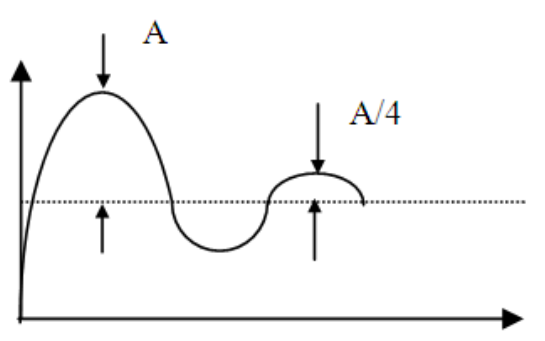
\includegraphics[width=0.5\linewidth]{Figuras/Ch14/fig1}
\end{frame}


\begin{frame}{Tentativa e erro}
	\begin{block}{Passo a passo}		
		Um procedimento típico de sintonia de controladores PID realizado em malha fechada é o seguinte:
		\begin{enumerate}
			\item Eliminar os termos integral e derivativo escolhendo $ \bm{T_i} $ com seu valor \textbf{máximo} e $ \bm{T_d} $ com seu valor \textbf{mínimo}.
			\item Atribuir a $ \bm{K_c} $ um valor \textbf{baixo} e colocar o controlador no modo \textbf{automático}.
			\item \textbf{Aumentar} o ganho $ \bm{K_c} $, em pequenos passos, até que ocorra uma oscilação \textbf{estável}, ou seja, com amplitude \textbf{constante}.			
			\item \textbf{Reduzir}, então, $ \bm{K_c} $ pela \textbf{metade}.		
			\item \textbf{Diminuir} $ \bm{T_i} $ \textbf{gradualmente} até observar novamente a ocorrência de uma oscilação \textbf{continuada}. Fixe então $ \bm{T_i} $ em \textbf{3 vezes este valor}.
			\item \textbf{Aumentar} $ \bm{T_d} $ também gradualmente até que ocorra novamente uma \textbf{oscilação mantida}. Faça então $ \bm{T_d} $ igual a $ \bm{1/3} $ deste valor.
		\end{enumerate}
	\end{block}
\end{frame}


\begin{frame}{Tentativa e erro}
	\begin{block}{Ganho supremo}
		\begin{enumerate}
			\item O valor de $ K_c $ que se obtém no passo 3 é chamado de \textbf{ganho supremo},
			denotado por $ \bm{K_u} $.
			\item Ao realizar o procedimento anterior, é importante que a saída do controlador
			\textbf{não se sature}.
			\item Se houver saturação, pode ocorrer uma oscilação estável ainda
			que $ K_c > K_u $.
		\end{enumerate}
	\end{block}
\end{frame}


\begin{frame}{Tentativa e erro}
	\centering
	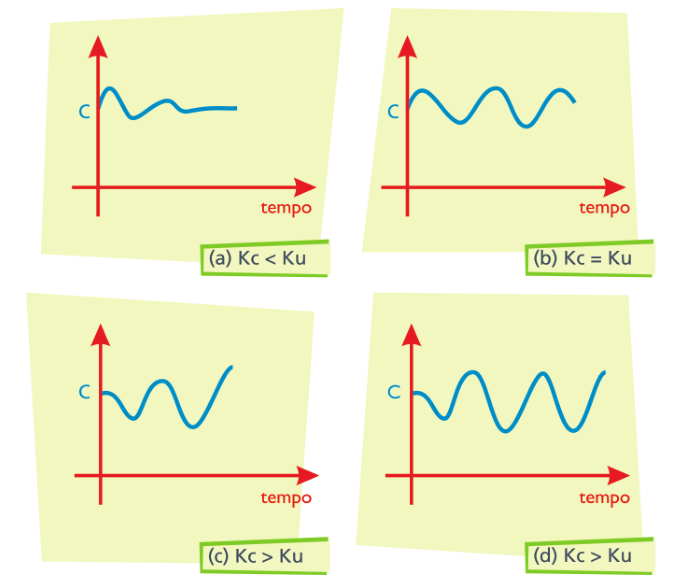
\includegraphics[width=0.7\linewidth]{Figuras/Ch14/fig2}
\end{frame}


\begin{frame}{Método de Ziegler-Nichols em malha fechada}
	\begin{block}{Introdução}
		\begin{itemize}
			\item Também conhecido como ``\textbf{segundo método de Ziegler-Nichols}'', trata-se de algo \textbf{similar à tentativa e erro}, porém mais \textbf{sistemático}.
			\item Nesse método, devemos encontrar $ K_u $ assim como descrito até o terceiro passo da tentativa e erro, assim como o \textbf{período de oscilação} do processo $ P_u $ (período crítico).
		\end{itemize}
	\end{block}

	\centering
	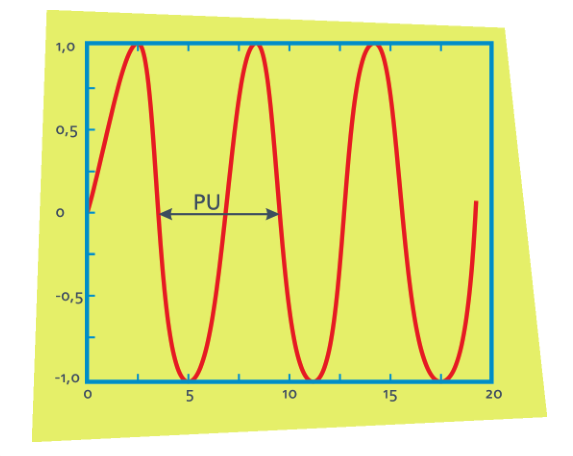
\includegraphics[width=0.5\linewidth]{Figuras/Ch14/fig3}
	
\end{frame}


\begin{frame}{Método de Ziegler-Nichols em malha fechada}
	\begin{block}{2º Ziegler-Nichols - Parâmetros para controladores}
		\resizebox{\textwidth}{!}{
			\begin{tabular}{cC{5em}C{5em}C{5em}}
				\toprule
				\thead{\normalsize Tipo do\\\normalsize controlador} & K_p & T_i & T_d\\ \midrule
				P & \num{0.5}\cdot K_u & - & - \\[0.2em]
				PI & \num{0.4}\cdot K_u & \num{0.8}\cdot P_u & - \\[0.2em]
				PID & \num{0.6}\cdot K_u & \num{0.5}\cdot P_u & \num{0.125}\cdot P_u \\ \bottomrule
		\end{tabular}}
	\end{block}
\end{frame}


\begin{frame}{Método de Ziegler-Nichols em malha fechada}
	\begin{block}{Exemplo \#01}
		\begin{itemize}
			\item Um técnico quer sintonizar um controlador num processo em \textbf{malha fechada} e decide usar o \textbf{2º método de Ziegler-Nichols} para tal.
			\item Primeiro faz o processo \textbf{oscilar}.
		\end{itemize}
	\end{block}
	
	\centering
	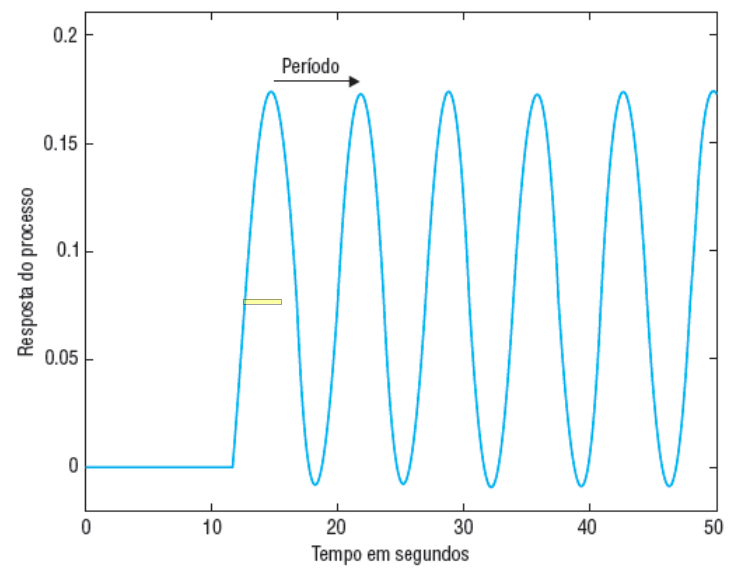
\includegraphics[width=0.55\linewidth]{Figuras/Ch14/fig3n2}
	
\end{frame}


\begin{frame}{Método de Ziegler-Nichols em malha fechada}
	\begin{block}{Exemplo \#01}
		\begin{itemize}
			\item De acordo com o programa que fornece o gráfico utilizado, $ P_u=\SI{4}{\second} $ e $ K_c=10 $ na condição de \textbf{oscilação}.
			\item Portanto, pela tabela, se deseja sintonizar um \textbf{controlador PI}, por exemplo, deve utilizar
			\begin{gather*}
			K_p=\num{0.4}\cdot K_u=\num{0.4}\cdot10=4\\
			T_i=\num{0.8}\cdot P_u=\num{0.8}\cdot4=\SI{3.2}{\second}
			\end{gather*}
		\end{itemize}
	\end{block}
\end{frame}


\begin{frame}{Sintonia em malha aberta}
	\begin{block}{Introdução - Função de transferência}
		\begin{itemize}
			\item Alguns métodos de sintonia analisam o comportamento do processo em \textbf{malha aberta}, aplicando uma \textbf{função degrau}, ou seja, que ``\textbf{pula}'' entre dois valores, por vezes de 0\% a 100\%.
			\item A partir da aplicação desse sinal e da análise da saída do processo, podemos analisar sua resposta em \textbf{curva característica} e, então, reduzí-lo à uma \textbf{função de primeiro grau com tempo morto}.
			\item Essa função trata-se de uma \textbf{função de transferência}, que é uma ferramenta analítica \textbf{muito útil} em controle.
			\item A função de transferência é uma \textbf{forma conveniente} de transcrever o \textbf{comportamento} do processo, e tem o seguinte formato:
			\[ G(s)=\dfrac{K\text{e}^{-Ls}}{Ts+1} \]
		\end{itemize}
	\end{block}
\end{frame}


\begin{frame}{Sintonia em malha aberta}
	\begin{block}{Resposta característica}
		\begin{itemize}
			\item Cada uma das constantes numa função de transferência tem um \textbf{significado físico} que pode ser encontrado no \textbf{gráfico} da \textbf{resposta característica} do processo.
		\end{itemize}
	\end{block}

	\centering
	\scalebox{1.2}{\begin{tikzpicture}[scale=0.5]
			\draw (-4,-3) rectangle (4,3); %CLP
		\draw (-4,0) -- (-2.5,0); %Div in out
		\draw (-2.5,-3) -- (-2.5,3); %Div cartoes
		\draw (-1.5,-2.5) rectangle (0,2.5); %Mem dados
		\draw (0.5,-2.5) rectangle (3.5,-1); %Mem prog
		\draw (1,0) rectangle (3,2); %CPU
		\draw (-4,-5) rectangle (4,-3); %Alimentacao
		\draw (-2.5,4) rectangle (4,6); %Term de prog
		
		\draw (1,2.6) node {CLP};
		
		\draw (-3.25,1.5) node[text width=1.5cm,align=center,rotate=90] {\small Cartões de input};
		
		\draw (-3.25,-1.5) node[text width=1.5cm,align=center,rotate=90] {\small Cartões de output};
		
		\node at (2,1) {\small CPU};
		
		\node[rotate=90,text width=1.5cm,align=center] at (-0.75,0) {\small Memória de dados};
		
		\node[text width=2cm,align=center] at (2,-1.75) {\footnotesize Memória de programa};
		
		\node at (-6,0) {Campo};
		
		\node at (0,-4) {Alimentação};
		
		\node[text width=3cm,align=center] at (0.75,5) {Terminal de programação};
		
		\draw[-Latex] (-8,1.5) -- node[above] {Entradas} +(4,0);
		\draw[Latex-] (-8,-1.5) -- node[below] {Saídas} +(4,0);
		\draw[-Latex] (-2.5,1.5) -- +(1,0);
		\draw[Latex-] (-2.5,-1.5) -- +(1,0);
		\draw[-Latex] (0,1.5) -- +(1,0);
		\draw[Latex-] (0,0.5) -- +(1,0);
		\draw[Latex-] (2,0) -- +(0,-1);
		
		\draw[-Latex] (-1.5,4) -- +(0,-1);
		\draw[Latex-] (3,4) -- +(0,-1);
	\end{tikzpicture}}
	
\end{frame}


\begin{frame}{Sintonia em malha aberta}
	\begin{block}{Constantes da função de transferência}
		\begin{itemize}
			\item $ L $ é o \textbf{tempo morto}.
			\item $ T $ é a \textbf{constante de tempo} (tempo necessário para o processo atingir \num{0.632} do valor final).
			\item $ V_f $ e $ V_i $ são os valores \textbf{final} e \textbf{inicial} do \textbf{processo} durante a aplicação do sinal em degrau.
		\end{itemize}
	\end{block}
	
	\centering
	\scalebox{1}{\begin{tikzpicture}[scale=0.5]
			\draw (-4,-3) rectangle (4,3); %CLP
		\draw (-4,0) -- (-2.5,0); %Div in out
		\draw (-2.5,-3) -- (-2.5,3); %Div cartoes
		\draw (-1.5,-2.5) rectangle (0,2.5); %Mem dados
		\draw (0.5,-2.5) rectangle (3.5,-1); %Mem prog
		\draw (1,0) rectangle (3,2); %CPU
		\draw (-4,-5) rectangle (4,-3); %Alimentacao
		\draw (-2.5,4) rectangle (4,6); %Term de prog
		
		\draw (1,2.6) node {CLP};
		
		\draw (-3.25,1.5) node[text width=1.5cm,align=center,rotate=90] {\small Cartões de input};
		
		\draw (-3.25,-1.5) node[text width=1.5cm,align=center,rotate=90] {\small Cartões de output};
		
		\node at (2,1) {\small CPU};
		
		\node[rotate=90,text width=1.5cm,align=center] at (-0.75,0) {\small Memória de dados};
		
		\node[text width=2cm,align=center] at (2,-1.75) {\footnotesize Memória de programa};
		
		\node at (-6,0) {Campo};
		
		\node at (0,-4) {Alimentação};
		
		\node[text width=3cm,align=center] at (0.75,5) {Terminal de programação};
		
		\draw[-Latex] (-8,1.5) -- node[above] {Entradas} +(4,0);
		\draw[Latex-] (-8,-1.5) -- node[below] {Saídas} +(4,0);
		\draw[-Latex] (-2.5,1.5) -- +(1,0);
		\draw[Latex-] (-2.5,-1.5) -- +(1,0);
		\draw[-Latex] (0,1.5) -- +(1,0);
		\draw[Latex-] (0,0.5) -- +(1,0);
		\draw[Latex-] (2,0) -- +(0,-1);
		
		\draw[-Latex] (-1.5,4) -- +(0,-1);
		\draw[Latex-] (3,4) -- +(0,-1);
	\end{tikzpicture}}
	
\end{frame}


\begin{frame}{Sintonia em malha aberta}
	\begin{block}{Ponto de inflexão}
		\begin{itemize}
			\item A linha a partir da qual determinamos os valores de $ L $ e $ T $ é a \textbf{extensão da tangente} no \textbf{ponto de inflexão} da curva de \textbf{resposta característica}.
			\item O \textbf{ponto de inflexão} de uma curva é o ponto exato onde a curva \textbf{muda a direção de mudança} (a variação estava crescendo e começa a diminuir).
			\item Podemos ver o ponto de inflexão, também, como o momento onde a \textbf{concavidade} da curva \textbf{se altera}.
		\end{itemize}
	\end{block}
\end{frame}


\begin{frame}{Sintonia em malha aberta}
	
	\centering
	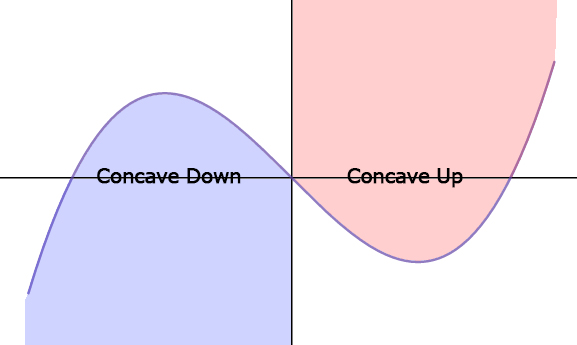
\includegraphics[width=0.9\linewidth]{Figuras/Ch14/fig6}
	
	\bigskip
	
	Visualização do ponto de inflexão
\end{frame}


\begin{frame}{Sintonia em malha aberta}
	\begin{block}{Primeiro método de Ziegler-Nichols}
		\begin{itemize}
			\item Um dos métodos utilizados para sintonizar controladores PID em malha aberta é o método de \textbf{Ziegler-Nichols em malha aberta}, também conhecido como \textbf{primeiro método de Ziegler-Nichols}.
			\item Consiste em, usando a função de transferência, encontrar o \textbf{ganho} e \textbf{tempos} do controlador utilizando dados \textbf{tabelados}.
			\item Sendo $ \Delta X $ a variação da entrada (função degrau) e $ \Delta VP $ a variação na saída do processo: \[ K=\dfrac{\Delta VP}{\Delta X} \]
		\end{itemize}
	\end{block}
\end{frame}


\begin{frame}{Sintonia em malha aberta}
	\begin{block}{1º Ziegler-Nichols - Parâmetros para controladores}
		\resizebox{\textwidth}{!}{
			\begin{tabular}{cC{7em}C{7em}C{7em}}
				\toprule
				\thead{\normalsize Tipo do\\\normalsize controlador} & K_p & T_i & T_d\\ \midrule
				P & \dfrac{T}{KL} & - & - \\[1em]
				PI & \num{0.9}\cdot\dfrac{T}{KL} & \num{3.3}\cdot L & - \\[1em]
				PID & \num{1.2}\cdot\dfrac{T}{KL} & 2\cdot L & \num{0.5}\cdot L \\ \bottomrule
		\end{tabular}}
	\end{block}
\end{frame}


\begin{frame}{Sintonia em malha aberta}
	\begin{block}{Primeiro método de Ziegler-Nichols - Exemplo \#01}
		\begin{itemize}
			\item Suponha que, numa fábrica de cola, a mistura que dá origem ao produto final deva ficar durante \SI{40}{\second} à uma temperatura de \SI{200}{\degreeCelsius} para adquirir a consistência desejada.
			\item Para que isso ocorra sem problemas, contratam dois técnicos em automação industrial, que devem encontrar os parâmetros para o controlador de temperatura do forno das colas.
			\item Os técnicos vão utilizar o \textbf{1º método de Ziegler-Nichols} para o trabalho.
		\end{itemize}
	\end{block}
\end{frame}


\begin{frame}{Sintonia em malha aberta}
	\centering
	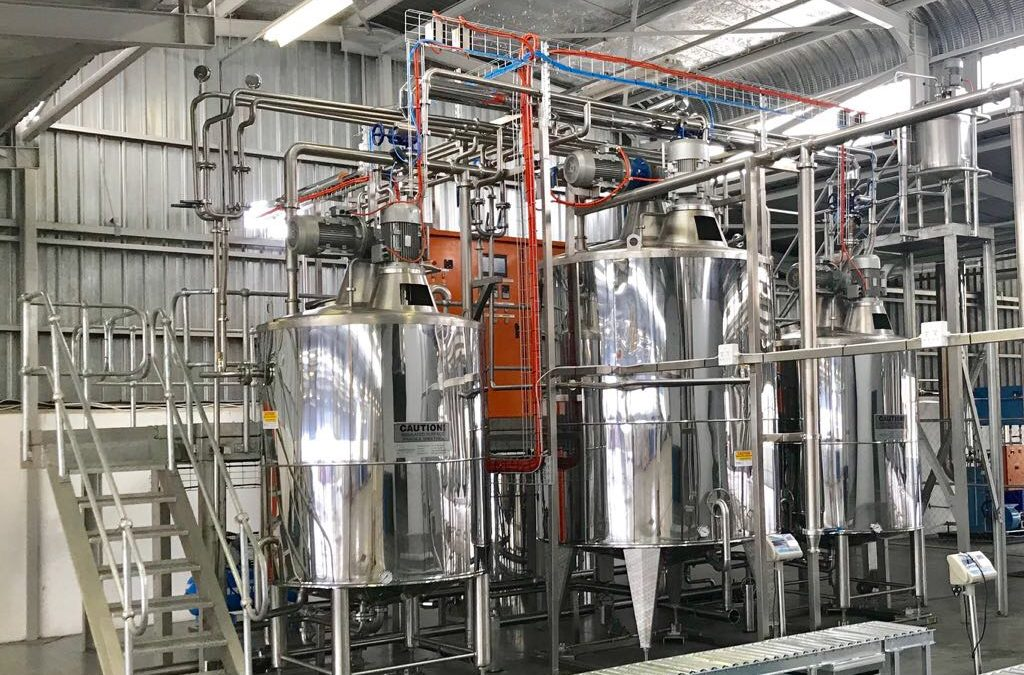
\includegraphics[width=0.9\linewidth]{Figuras/Ch14/fig6n2}
\end{frame}


\begin{frame}{Sintonia em malha aberta}
	\begin{block}{Primeiro método de Ziegler-Nichols - Exemplo \#01}
		\begin{itemize}
			\item A \textbf{curva característica} do processo encontrada para uma entrada $ \Delta X=5\% $ está ilustrada abaixo.
		\end{itemize}
	\end{block}
	
	\centering
	\scalebox{1.3}{

\tikzset{every picture/.style={line width=0.75pt}} %set default line width to 0.75pt        

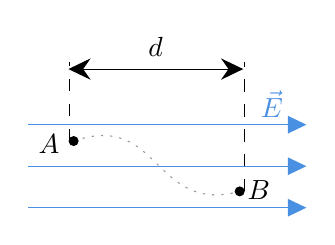
\begin{tikzpicture}[x=0.75pt,y=0.75pt,yscale=-1,xscale=1]
%uncomment if require: \path (0,300); %set diagram left start at 0, and has height of 300

%Curve Lines [id:da6177490068384819] 
\draw [color={rgb, 255:red, 155; green, 155; blue, 155 }  ,draw opacity=1 ] [dash pattern={on 0.84pt off 2.51pt}]  (137.88,127.88) .. controls (180,113.4) and (176,163.4) .. (217.88,152.13) ;


%Straight Lines [id:da7124330895115376] 
\draw [color={rgb, 255:red, 74; green, 144; blue, 226 }  ,draw opacity=1 ]   (116,120) -- (247,120) ;
\draw [shift={(250,120)}, rotate = 180] [fill={rgb, 255:red, 74; green, 144; blue, 226 }  ,fill opacity=1 ][line width=0.08]  [draw opacity=0] (8.93,-4.29) -- (0,0) -- (8.93,4.29) -- cycle    ;

%Straight Lines [id:da12792354611605283] 
\draw [color={rgb, 255:red, 74; green, 144; blue, 226 }  ,draw opacity=1 ]   (116,140) -- (247,140) ;
\draw [shift={(250,140)}, rotate = 180] [fill={rgb, 255:red, 74; green, 144; blue, 226 }  ,fill opacity=1 ][line width=0.08]  [draw opacity=0] (8.93,-4.29) -- (0,0) -- (8.93,4.29) -- cycle    ;

%Straight Lines [id:da4044562129660001] 
\draw [color={rgb, 255:red, 74; green, 144; blue, 226 }  ,draw opacity=1 ]   (116,160) -- (247,160) ;
\draw [shift={(250,160)}, rotate = 180] [fill={rgb, 255:red, 74; green, 144; blue, 226 }  ,fill opacity=1 ][line width=0.08]  [draw opacity=0] (8.93,-4.29) -- (0,0) -- (8.93,4.29) -- cycle    ;

%Shape: Circle [id:dp28224868607946574] 
\draw  [fill={rgb, 255:red, 0; green, 0; blue, 0 }  ,fill opacity=1 ] (135.75,127.88) .. controls (135.75,126.7) and (136.7,125.75) .. (137.88,125.75) .. controls (139.05,125.75) and (140,126.7) .. (140,127.88) .. controls (140,129.05) and (139.05,130) .. (137.88,130) .. controls (136.7,130) and (135.75,129.05) .. (135.75,127.88) -- cycle ;
%Shape: Circle [id:dp03942976292609046] 
\draw  [color={rgb, 255:red, 0; green, 0; blue, 0 }  ,draw opacity=1 ][fill={rgb, 255:red, 0; green, 0; blue, 0 }  ,fill opacity=1 ] (215.75,152.13) .. controls (215.75,150.95) and (216.7,150) .. (217.88,150) .. controls (219.05,150) and (220,150.95) .. (220,152.13) .. controls (220,153.3) and (219.05,154.25) .. (217.88,154.25) .. controls (216.7,154.25) and (215.75,153.3) .. (215.75,152.13) -- cycle ;
%Straight Lines [id:da5788684610773114] 
\draw  [dash pattern={on 4.5pt off 4.5pt}]  (135.75,127.88) -- (135.75,90) ;


%Straight Lines [id:da7063621547892809] 
\draw  [dash pattern={on 4.5pt off 4.5pt}]  (220,152.13) -- (220,90) ;


%Straight Lines [id:da8063380246624134] 
\draw    (138.35,93.2) -- (216.6,93.2) ;
\draw [shift={(219.6,93.2)}, rotate = 180] [fill={rgb, 255:red, 0; green, 0; blue, 0 }  ][line width=0.08]  [draw opacity=0] (10.72,-5.15) -- (0,0) -- (10.72,5.15) -- (7.12,0) -- cycle    ;
\draw [shift={(135.35,93.2)}, rotate = 0] [fill={rgb, 255:red, 0; green, 0; blue, 0 }  ][line width=0.08]  [draw opacity=0] (10.72,-5.15) -- (0,0) -- (10.72,5.15) -- (7.12,0) -- cycle    ;

% Text Node
\draw (233.4,110) node [color={rgb, 255:red, 74; green, 144; blue, 226 }  ,opacity=1 ]  {$\vec{E}$};
% Text Node
\draw (177.33,82.33) node   {$d$};
% Text Node
\draw (126,129.33) node   {$A$};
% Text Node
\draw (227.13,151.4) node   {$B$};


\end{tikzpicture}
}
	
\end{frame}


\begin{frame}{Sintonia em malha aberta}
	\begin{block}{Primeiro método de Ziegler-Nichols - Exemplo \#01}
		\begin{itemize}
			\item Utilizando \[ K=\dfrac{\Delta VP}{\Delta X}=\dfrac{51\%-45\%}{5\%}=\dfrac{6\%}{5\%}=\num{1.2} \]
			os técnicos encontram a \textbf{função de transferência de 1ª ordem} do processo \[ G(s)=\dfrac{\num{1.2}
				\text{e}^{-s}}{2s+1} \]
			\item A partir desta, podem sintonizar o \textbf{controlador PID} da fábrica, utilizando os parâmetros
			\begin{gather*}
			K_p=\num{1.2}\cdot\dfrac{T}{KL}=\num{1,2}\cdot\dfrac{2}{\num{1.2}\cdot1}=2\\
			T_i=2\cdot L=2\cdot1=\SI{2}{\second}\\
			T_d=\num{0.5}\cdot L=\num{0.5}\cdot1=\SI{0.5}{\second}
			\end{gather*}
		\end{itemize}
	\end{block}
\end{frame}


\begin{frame}{Sintonia em malha aberta}
	\begin{block}{Primeiro método de Ziegler-Nichols - Exemplo \#02}
		\begin{itemize}
			\item A \textbf{curva característica} do processo encontrada para uma entrada $ \Delta X=1 $ (degrau unitário) está ilustrada abaixo.
		\end{itemize}
	\end{block}
	
	\centering
	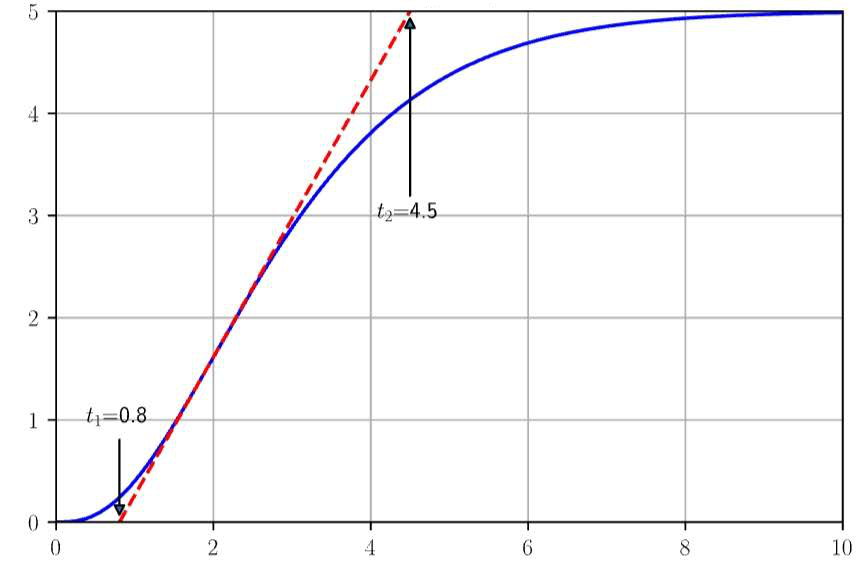
\includegraphics[width=0.7\linewidth]{Figuras/Ch14/fig3n3}
	
\end{frame}


\begin{frame}{Sintonia em malha aberta}
	\begin{block}{Primeiro método de Ziegler-Nichols - Exemplo \#02}
		\begin{itemize}
			\item Utilizando \[ K=\dfrac{\Delta VP}{\Delta X}=\dfrac{5-0}{1}=5 \] e fazendo $ L=\SI{0.8}{\second} $ e $ T=t_2-L=\SI{4.5}{\second}-\SI{0.8}{\second}=\SI{3.7}{\second} $
			temos \[ G(s)=\dfrac{5
				\text{e}^{-\num{0.8}s}}{\num{3.7}s+1} \]
			\item A partir desta, um \textbf{controlador PI} pode ser sintonizado utilizando os parâmetros
			\begin{gather*}
			K_p=\num{0.9}\cdot\dfrac{T}{KL}=\num{0.9}\cdot\dfrac{\num{3.7}}{\num{5}\cdot\num{0.8}}=\num{0.9}\cdot\num{0.925}=\num{0.8325}\\
			T_i=\num{3.3}\cdot L=\num{3.3}\cdot\num{0.8}=\SI{2.64}{\second}
			\end{gather*}
		\end{itemize}
	\end{block}
\end{frame}


\begin{frame}{Sintonia em malha aberta}
	\begin{block}{Método de Cohen-Coon}
		\begin{itemize}
			\item O método de sintonia \textbf{Cohen-Coon} é \textbf{mais geral} do que o de Ziegler-Nichols em malha aberta.
			\item Ziegler-Nichols funciona somente para processos onde o tempo morto é \textbf{metade} da constante de tempo.
			\item Cohen-Coon consegue transpor essa dificuldade, podendo se estender mais até do que com o tempo morto sendo o \textbf{dobro} da constante de tempo.
			\item O método Cohen-Coon também é capaz de sintonizar controladores PD.
		\end{itemize}
	\end{block}
\end{frame}


\begin{frame}{Sintonia em malha aberta}
	\begin{block}{Constantes da função de transferência}
		\begin{itemize}
			\item No método Cohen-Coon devemos encontrar as constantes da função de transferência através dos valores abaixo.
		\end{itemize}
	\end{block}
	
	\centering
	\scalebox{1.5}{\newcommand{\innercolor}{gray!70!white}
	\newcommand{\outercolor}{gray!40!white}
	\newcommand{\leftcoil}{red!75!gray}
	\pgfmathsetmacro{\coilseparation}{0.02}
	
	\pgfmathsetmacro{\halflinewidth}{0.008}
	
	
	\begin{tikzpicture}[x={(\xx*1cm,\xy*1cm)},y={(\yx*1cm,\yy*1cm)},z={(\zx*1cm,\zy*1cm)}]
	\draw[\leftcoil, thick] (-0.02,5,1.125) -- +(0,2,0) (1.02,5,3.875) -- +(0,2,0);
	
	\draw[dashed,<->] ($ (-0.02,5,1.125)+(0,2,0) $) -- ($ (1.02,5,3.875)+(0,2,0) $);
	\node[rotate=85] at ($ (-0.02,5+2,1.125)!0.5!(1.02,5+2,3.875)+(0,0.2,0) $) {$ V_p $};
	
	\draw[-latex] (-0.02,6.5,1.325) -- node[above] {$ i_p $} +(0,-1,0);
	\draw[latex-] (1.02,0.02-0.5,1.3) -- node[above] {$ i_s $} +(0,-1,0);
	
	\filldraw[fill=\innercolor]  (0,1,1) -- (1,1,1) -- (1,4,1) -- (0,4,1) -- cycle;
	\filldraw[fill=\innercolor]  (1,4,1) -- (0,4,1) -- (0,4,4) -- (1,4,4) -- cycle;
	\filldraw[fill=\innercolor]  (0,0,0) -- (1,0,0) -- (1,0,5) -- (0,0,5) -- cycle;
	\filldraw[fill=\innercolor]  (0,0,5) -- (0,5,5) -- (1,5,5) -- (1,0,5) -- cycle;
	\filldraw[fill=\outercolor,even odd rule]    (0,0,0) -- (0,5,0) -- (0,5,5) -- (0,0,5) --cycle (0,1,1) -- (0,4,1) -- (0,4,4) -- (0,1,4) --cycle ;
	
	\begin{scope}
	\clip (0,3,1) -- (0,6,1) -- (0,6,4) -- (0,3,4);
	\foreach \z in {1.125,1.375,...,3.875}
	{   \draw[\leftcoil,thick] (0,5,\z) -- (-\coilseparation,5,\z) -- (-\coilseparation,4-\coilseparation,\z) -- (1+\coilseparation,4-\coilseparation,\z) -- (1+\coilseparation,4,\z);
	}
	\end{scope}
	
	
	\foreach \z in {1.25,1.75,...,3.75}
	{   \draw[blue,thick] (0,1,\z) -- (-\coilseparation,1,\z) -- (-\coilseparation,0-\coilseparation,\z) -- (1+\coilseparation,0-\coilseparation,\z) -- (1+\coilseparation,0,\z);
	}

	\draw[blue,thick] (1+\coilseparation,0+\coilseparation,1.1) -- +(0,-2,0) (-\coilseparation,1+\coilseparation,3.85) -- +(0,-3,0);
	
	\draw[dashed,<->] (1.02,-2+0.02,1.1) -- (-0.02,0.02-2,3.85);
	\node[rotate=-70] at ($ (1.02,-2+0.02,1.1)!0.5!(-0.02,0.02-2,3.85)+(0,-0.2,0) $) {$ V_s $};
	
	\draw[decorate,decoration={brace,amplitude=10pt},xshift=-4pt,yshift=0pt] (0,5,1.25) -- +(0,0,2.75);
	\draw[decorate,decoration={brace,amplitude=10pt},xshift=-4pt,yshift=0pt] (1.2,0,3.75) -- +(0,0,-2.6);
	\node[rotate=90] at (0,5.7,2.625) {$ N_p $ espiras};
	\node[rotate=-90] at (1.2,-0.5,2.5) {$ N_s $ espiras};
	
	\draw[dashed,postaction={decorate,decoration={markings,mark=between positions 0.1 and 1 step 0.2 with \arrow{Latex}}}] (0,4.5,0.5) -- (0,0.5,0.5) -- ++(0,0,4) -- ++(0,4,0) -- cycle;
	
	\draw[] (0,2.5,4.7)% -- +(0,-0.5,1.5)
	node[rotate=-10] {Fluxo magnético ($ \phi $)};
	
	\end{tikzpicture}}
	
\end{frame}


\begin{frame}{Sintonia em malha aberta}
	\begin{block}{Constantes da função de transferência}
		\begin{itemize}
			\item $ T=\dfrac{3}{2}\del{t_2-t_1} $.
			\item $ L=t_2-T $
		\end{itemize}
	\end{block}
	
	\centering
	\scalebox{1.4}{\newcommand{\innercolor}{gray!70!white}
	\newcommand{\outercolor}{gray!40!white}
	\newcommand{\leftcoil}{red!75!gray}
	\pgfmathsetmacro{\coilseparation}{0.02}
	
	\pgfmathsetmacro{\halflinewidth}{0.008}
	
	
	\begin{tikzpicture}[x={(\xx*1cm,\xy*1cm)},y={(\yx*1cm,\yy*1cm)},z={(\zx*1cm,\zy*1cm)}]
	\draw[\leftcoil, thick] (-0.02,5,1.125) -- +(0,2,0) (1.02,5,3.875) -- +(0,2,0);
	
	\draw[dashed,<->] ($ (-0.02,5,1.125)+(0,2,0) $) -- ($ (1.02,5,3.875)+(0,2,0) $);
	\node[rotate=85] at ($ (-0.02,5+2,1.125)!0.5!(1.02,5+2,3.875)+(0,0.2,0) $) {$ V_p $};
	
	\draw[-latex] (-0.02,6.5,1.325) -- node[above] {$ i_p $} +(0,-1,0);
	\draw[latex-] (1.02,0.02-0.5,1.3) -- node[above] {$ i_s $} +(0,-1,0);
	
	\filldraw[fill=\innercolor]  (0,1,1) -- (1,1,1) -- (1,4,1) -- (0,4,1) -- cycle;
	\filldraw[fill=\innercolor]  (1,4,1) -- (0,4,1) -- (0,4,4) -- (1,4,4) -- cycle;
	\filldraw[fill=\innercolor]  (0,0,0) -- (1,0,0) -- (1,0,5) -- (0,0,5) -- cycle;
	\filldraw[fill=\innercolor]  (0,0,5) -- (0,5,5) -- (1,5,5) -- (1,0,5) -- cycle;
	\filldraw[fill=\outercolor,even odd rule]    (0,0,0) -- (0,5,0) -- (0,5,5) -- (0,0,5) --cycle (0,1,1) -- (0,4,1) -- (0,4,4) -- (0,1,4) --cycle ;
	
	\begin{scope}
	\clip (0,3,1) -- (0,6,1) -- (0,6,4) -- (0,3,4);
	\foreach \z in {1.125,1.375,...,3.875}
	{   \draw[\leftcoil,thick] (0,5,\z) -- (-\coilseparation,5,\z) -- (-\coilseparation,4-\coilseparation,\z) -- (1+\coilseparation,4-\coilseparation,\z) -- (1+\coilseparation,4,\z);
	}
	\end{scope}
	
	
	\foreach \z in {1.25,1.75,...,3.75}
	{   \draw[blue,thick] (0,1,\z) -- (-\coilseparation,1,\z) -- (-\coilseparation,0-\coilseparation,\z) -- (1+\coilseparation,0-\coilseparation,\z) -- (1+\coilseparation,0,\z);
	}

	\draw[blue,thick] (1+\coilseparation,0+\coilseparation,1.1) -- +(0,-2,0) (-\coilseparation,1+\coilseparation,3.85) -- +(0,-3,0);
	
	\draw[dashed,<->] (1.02,-2+0.02,1.1) -- (-0.02,0.02-2,3.85);
	\node[rotate=-70] at ($ (1.02,-2+0.02,1.1)!0.5!(-0.02,0.02-2,3.85)+(0,-0.2,0) $) {$ V_s $};
	
	\draw[decorate,decoration={brace,amplitude=10pt},xshift=-4pt,yshift=0pt] (0,5,1.25) -- +(0,0,2.75);
	\draw[decorate,decoration={brace,amplitude=10pt},xshift=-4pt,yshift=0pt] (1.2,0,3.75) -- +(0,0,-2.6);
	\node[rotate=90] at (0,5.7,2.625) {$ N_p $ espiras};
	\node[rotate=-90] at (1.2,-0.5,2.5) {$ N_s $ espiras};
	
	\draw[dashed,postaction={decorate,decoration={markings,mark=between positions 0.1 and 1 step 0.2 with \arrow{Latex}}}] (0,4.5,0.5) -- (0,0.5,0.5) -- ++(0,0,4) -- ++(0,4,0) -- cycle;
	
	\draw[] (0,2.5,4.7)% -- +(0,-0.5,1.5)
	node[rotate=-10] {Fluxo magnético ($ \phi $)};
	
	\end{tikzpicture}}
\end{frame}


\begin{frame}{Sintonia em malha aberta}
	\begin{block}{Cohen-Coon - Parâmetros para controladores}
		\centering
		\begin{adjustbox}{totalheight=0.89\textheight-2\baselineskip}
			\begin{tabular}{cC{5em}C{5em}C{5em}}
				\toprule
				\thead{\normalsize Tipo do\\\normalsize controlador} & K_p & T_i & T_d\\ \midrule
				P 	& \dfrac{T}{KL}\del{1+\dfrac{L}{3T}} & - & - \\[0.5em]
				PI 	& \dfrac{T}{KL}\del{\num{0.9}+\dfrac{L}{12T}} & L\del{\dfrac{30+\dfrac{3L}{T}}{9+\dfrac{20L}{T}}} & - \\[0.5em]
				PD	& \dfrac{T}{KL}\del{\num{1.25}+\dfrac{L}{6T}} & - & L\del{\dfrac{6-\dfrac{2L}{T}}{22+\dfrac{3L}{T}}} \\[2em]
				PID & \dfrac{T}{KL}\del{\num{1.33}+\dfrac{L}{4T}} & L\del{\dfrac{32+\dfrac{6L}{T}}{13+\dfrac{8L}{T}}} & L\del{\dfrac{4}{11+\dfrac{2L}{T}}} \\ \bottomrule
			\end{tabular}
		\end{adjustbox}
	\end{block}
\end{frame}


\begin{frame}{Sintonia em malha aberta}
	\begin{block}{Método de Cohen-Coon - Exemplo \#01}
		\begin{itemize}
			\item Uma máquina de pintura de automóveis deve ter seu \textbf{controlador PD} sintonizado, para isso o técnico da fábrica utiliza o \textbf{método de Cohen-Coon}.
			\item Aplicando uma entrada $ \Delta X=12\% $, encontra o seguinte gráfico.
		\end{itemize}
	\end{block}
	
	\centering
	\scalebox{1.3}{

\tikzset{every picture/.style={line width=0.75pt}} %set default line width to 0.75pt        

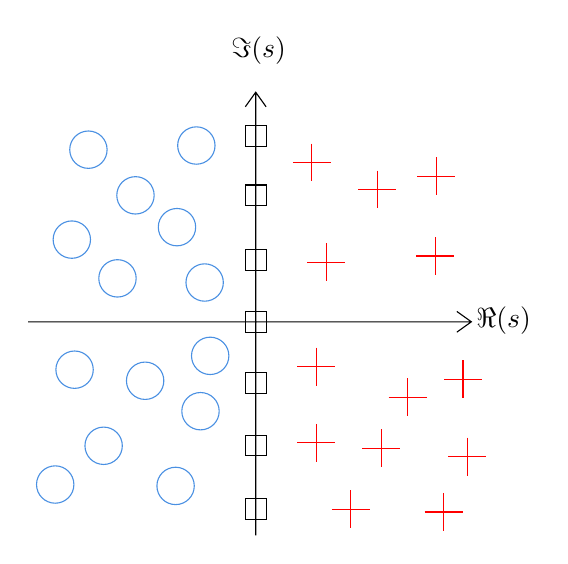
\begin{tikzpicture}[x=0.75pt,y=0.75pt,yscale=-1,xscale=1]
%uncomment if require: \path (0,300); %set diagram left start at 0, and has height of 300

%Shape: Axis 2D [id:dp27678030181731494] 
\draw  (40,160.6) -- (253.5,160.6)(149.6,50) -- (149.6,263.5) (246.5,155.6) -- (253.5,160.6) -- (246.5,165.6) (144.6,57) -- (149.6,50) -- (154.6,57)  ;
%Shape: Square [id:dp29640104318485094] 
\draw   (144.6,155.6) -- (154.6,155.6) -- (154.6,165.6) -- (144.6,165.6) -- cycle ;
%Shape: Square [id:dp5015049228757054] 
\draw   (144.6,125.7) -- (154.6,125.7) -- (154.6,135.7) -- (144.6,135.7) -- cycle ;
%Shape: Square [id:dp5724308304859749] 
\draw   (144.6,94.7) -- (154.6,94.7) -- (154.6,104.7) -- (144.6,104.7) -- cycle ;
%Shape: Square [id:dp8722658997981245] 
\draw   (144.6,66.2) -- (154.6,66.2) -- (154.6,76.2) -- (144.6,76.2) -- cycle ;
%Shape: Square [id:dp035501458242915174] 
\draw   (144.6,185.2) -- (154.6,185.2) -- (154.6,195.2) -- (144.6,195.2) -- cycle ;
%Shape: Square [id:dp23226558696093957] 
\draw   (144.6,215.2) -- (154.6,215.2) -- (154.6,225.2) -- (144.6,225.2) -- cycle ;
%Shape: Square [id:dp09667812864869552] 
\draw   (144.6,245.7) -- (154.6,245.7) -- (154.6,255.7) -- (144.6,255.7) -- cycle ;
\draw  [color={rgb, 255:red, 255; green, 0; blue, 0 }  ,draw opacity=1 ] (167.5,83.88) -- (185.75,83.88)(176.63,74.75) -- (176.63,93) ;
\draw  [color={rgb, 255:red, 255; green, 0; blue, 0 }  ,draw opacity=1 ] (199,96.88) -- (217.25,96.88)(208.13,87.75) -- (208.13,106) ;
\draw  [color={rgb, 255:red, 255; green, 0; blue, 0 }  ,draw opacity=1 ] (174.5,131.88) -- (192.75,131.88)(183.63,122.75) -- (183.63,141) ;
\draw  [color={rgb, 255:red, 255; green, 0; blue, 0 }  ,draw opacity=1 ] (227,128.88) -- (245.25,128.88)(236.13,119.75) -- (236.13,138) ;
\draw  [color={rgb, 255:red, 255; green, 0; blue, 0 }  ,draw opacity=1 ] (227.5,90.38) -- (245.75,90.38)(236.63,81.25) -- (236.63,99.5) ;
\draw  [color={rgb, 255:red, 255; green, 0; blue, 0 }  ,draw opacity=1 ] (169.67,182.21) -- (187.92,182.21)(178.79,173.08) -- (178.79,191.33) ;
\draw  [color={rgb, 255:red, 255; green, 0; blue, 0 }  ,draw opacity=1 ] (186.33,250.88) -- (204.58,250.88)(195.46,241.75) -- (195.46,260) ;
\draw  [color={rgb, 255:red, 255; green, 0; blue, 0 }  ,draw opacity=1 ] (231,252.21) -- (249.25,252.21)(240.13,243.08) -- (240.13,261.33) ;
\draw  [color={rgb, 255:red, 255; green, 0; blue, 0 }  ,draw opacity=1 ] (169.67,218.88) -- (187.92,218.88)(178.79,209.75) -- (178.79,228) ;
\draw  [color={rgb, 255:red, 255; green, 0; blue, 0 }  ,draw opacity=1 ] (242.33,225.54) -- (260.58,225.54)(251.46,216.42) -- (251.46,234.67) ;
\draw  [color={rgb, 255:red, 255; green, 0; blue, 0 }  ,draw opacity=1 ] (213.67,196.88) -- (231.92,196.88)(222.79,187.75) -- (222.79,206) ;
\draw  [color={rgb, 255:red, 255; green, 0; blue, 0 }  ,draw opacity=1 ] (240.33,188.21) -- (258.58,188.21)(249.46,179.08) -- (249.46,197.33) ;
\draw  [color={rgb, 255:red, 255; green, 0; blue, 0 }  ,draw opacity=1 ] (201,221.54) -- (219.25,221.54)(210.13,212.42) -- (210.13,230.67) ;
%Shape: Circle [id:dp01739200493370019] 
\draw  [color={rgb, 255:red, 74; green, 144; blue, 226 }  ,draw opacity=1 ] (60,77.67) .. controls (60,72.7) and (64.03,68.67) .. (69,68.67) .. controls (73.97,68.67) and (78,72.7) .. (78,77.67) .. controls (78,82.64) and (73.97,86.67) .. (69,86.67) .. controls (64.03,86.67) and (60,82.64) .. (60,77.67) -- cycle ;
%Shape: Circle [id:dp857755141402053] 
\draw  [color={rgb, 255:red, 74; green, 144; blue, 226 }  ,draw opacity=1 ] (82.67,99.67) .. controls (82.67,94.7) and (86.7,90.67) .. (91.67,90.67) .. controls (96.64,90.67) and (100.67,94.7) .. (100.67,99.67) .. controls (100.67,104.64) and (96.64,108.67) .. (91.67,108.67) .. controls (86.7,108.67) and (82.67,104.64) .. (82.67,99.67) -- cycle ;
%Shape: Circle [id:dp9246833060771249] 
\draw  [color={rgb, 255:red, 74; green, 144; blue, 226 }  ,draw opacity=1 ] (44,239) .. controls (44,234.03) and (48.03,230) .. (53,230) .. controls (57.97,230) and (62,234.03) .. (62,239) .. controls (62,243.97) and (57.97,248) .. (53,248) .. controls (48.03,248) and (44,243.97) .. (44,239) -- cycle ;
%Shape: Circle [id:dp8304441936419562] 
\draw  [color={rgb, 255:red, 74; green, 144; blue, 226 }  ,draw opacity=1 ] (118.67,177) .. controls (118.67,172.03) and (122.7,168) .. (127.67,168) .. controls (132.64,168) and (136.67,172.03) .. (136.67,177) .. controls (136.67,181.97) and (132.64,186) .. (127.67,186) .. controls (122.7,186) and (118.67,181.97) .. (118.67,177) -- cycle ;
%Shape: Circle [id:dp5059258663614863] 
\draw  [color={rgb, 255:red, 74; green, 144; blue, 226 }  ,draw opacity=1 ] (102.67,115) .. controls (102.67,110.03) and (106.7,106) .. (111.67,106) .. controls (116.64,106) and (120.67,110.03) .. (120.67,115) .. controls (120.67,119.97) and (116.64,124) .. (111.67,124) .. controls (106.7,124) and (102.67,119.97) .. (102.67,115) -- cycle ;
%Shape: Circle [id:dp21245040687156935] 
\draw  [color={rgb, 255:red, 74; green, 144; blue, 226 }  ,draw opacity=1 ] (52,121) .. controls (52,116.03) and (56.03,112) .. (61,112) .. controls (65.97,112) and (70,116.03) .. (70,121) .. controls (70,125.97) and (65.97,130) .. (61,130) .. controls (56.03,130) and (52,125.97) .. (52,121) -- cycle ;
%Shape: Circle [id:dp17429736806925722] 
\draw  [color={rgb, 255:red, 74; green, 144; blue, 226 }  ,draw opacity=1 ] (116,141.67) .. controls (116,136.7) and (120.03,132.67) .. (125,132.67) .. controls (129.97,132.67) and (134,136.7) .. (134,141.67) .. controls (134,146.64) and (129.97,150.67) .. (125,150.67) .. controls (120.03,150.67) and (116,146.64) .. (116,141.67) -- cycle ;
%Shape: Circle [id:dp33160849295458217] 
\draw  [color={rgb, 255:red, 74; green, 144; blue, 226 }  ,draw opacity=1 ] (74,139.67) .. controls (74,134.7) and (78.03,130.67) .. (83,130.67) .. controls (87.97,130.67) and (92,134.7) .. (92,139.67) .. controls (92,144.64) and (87.97,148.67) .. (83,148.67) .. controls (78.03,148.67) and (74,144.64) .. (74,139.67) -- cycle ;
%Shape: Circle [id:dp32709834546378724] 
\draw  [color={rgb, 255:red, 74; green, 144; blue, 226 }  ,draw opacity=1 ] (87.33,189) .. controls (87.33,184.03) and (91.36,180) .. (96.33,180) .. controls (101.3,180) and (105.33,184.03) .. (105.33,189) .. controls (105.33,193.97) and (101.3,198) .. (96.33,198) .. controls (91.36,198) and (87.33,193.97) .. (87.33,189) -- cycle ;
%Shape: Circle [id:dp8791724327388495] 
\draw  [color={rgb, 255:red, 74; green, 144; blue, 226 }  ,draw opacity=1 ] (53.33,183.67) .. controls (53.33,178.7) and (57.36,174.67) .. (62.33,174.67) .. controls (67.3,174.67) and (71.33,178.7) .. (71.33,183.67) .. controls (71.33,188.64) and (67.3,192.67) .. (62.33,192.67) .. controls (57.36,192.67) and (53.33,188.64) .. (53.33,183.67) -- cycle ;
%Shape: Circle [id:dp4794866171308949] 
\draw  [color={rgb, 255:red, 74; green, 144; blue, 226 }  ,draw opacity=1 ] (114,203.67) .. controls (114,198.7) and (118.03,194.67) .. (123,194.67) .. controls (127.97,194.67) and (132,198.7) .. (132,203.67) .. controls (132,208.64) and (127.97,212.67) .. (123,212.67) .. controls (118.03,212.67) and (114,208.64) .. (114,203.67) -- cycle ;
%Shape: Circle [id:dp5349657045143856] 
\draw  [color={rgb, 255:red, 74; green, 144; blue, 226 }  ,draw opacity=1 ] (67.33,220.33) .. controls (67.33,215.36) and (71.36,211.33) .. (76.33,211.33) .. controls (81.3,211.33) and (85.33,215.36) .. (85.33,220.33) .. controls (85.33,225.3) and (81.3,229.33) .. (76.33,229.33) .. controls (71.36,229.33) and (67.33,225.3) .. (67.33,220.33) -- cycle ;
%Shape: Circle [id:dp714149478603834] 
\draw  [color={rgb, 255:red, 74; green, 144; blue, 226 }  ,draw opacity=1 ] (102,239.67) .. controls (102,234.7) and (106.03,230.67) .. (111,230.67) .. controls (115.97,230.67) and (120,234.7) .. (120,239.67) .. controls (120,244.64) and (115.97,248.67) .. (111,248.67) .. controls (106.03,248.67) and (102,244.64) .. (102,239.67) -- cycle ;
%Shape: Circle [id:dp476022910470574] 
\draw  [color={rgb, 255:red, 74; green, 144; blue, 226 }  ,draw opacity=1 ] (112,75.67) .. controls (112,70.7) and (116.03,66.67) .. (121,66.67) .. controls (125.97,66.67) and (130,70.7) .. (130,75.67) .. controls (130,80.64) and (125.97,84.67) .. (121,84.67) .. controls (116.03,84.67) and (112,80.64) .. (112,75.67) -- cycle ;

% Text Node
\draw (151,30) node   {$\Im(s)$};
% Text Node
\draw (269,160) node   {$\Re(s)$};


\end{tikzpicture}}
\end{frame}


\begin{frame}{Sintonia em malha aberta}
	\centering
	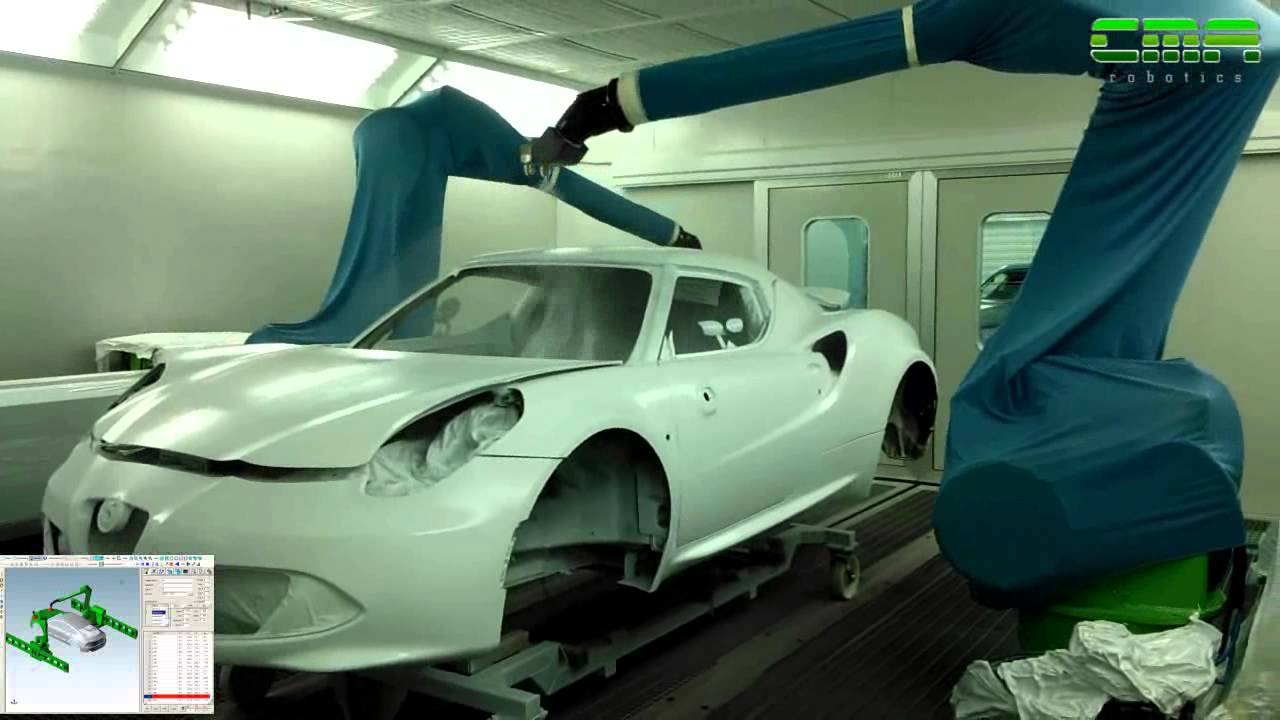
\includegraphics[width=0.9\linewidth]{Figuras/Ch14/fig6n3}
\end{frame}


\begin{frame}{Sintonia em malha aberta}
	\begin{block}{Método de Cohen-Coon - Exemplo \#01}
		\begin{itemize}
			\item $ T=\dfrac{3}{2}\del{\SI{4.5}{\second}-\SI{3}{\second}}=\dfrac{3}{2}\cdot\SI{1.5}{\second}=\SI{2.25}{\second} $.
			\item $ L=\SI{4.5}{\second}-\SI{2.25}{\second}=\SI{2.25}{\second} $
		\end{itemize}
	\end{block}
	
	\centering
	\scalebox{1.4}{

\tikzset{every picture/.style={line width=0.75pt}} %set default line width to 0.75pt        

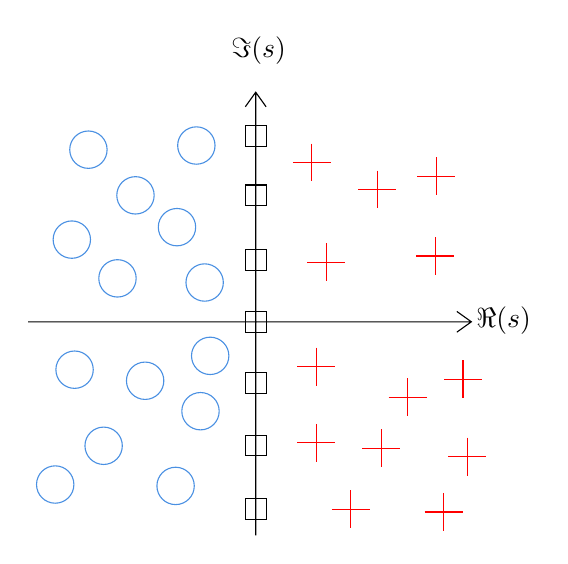
\begin{tikzpicture}[x=0.75pt,y=0.75pt,yscale=-1,xscale=1]
%uncomment if require: \path (0,300); %set diagram left start at 0, and has height of 300

%Shape: Axis 2D [id:dp27678030181731494] 
\draw  (40,160.6) -- (253.5,160.6)(149.6,50) -- (149.6,263.5) (246.5,155.6) -- (253.5,160.6) -- (246.5,165.6) (144.6,57) -- (149.6,50) -- (154.6,57)  ;
%Shape: Square [id:dp29640104318485094] 
\draw   (144.6,155.6) -- (154.6,155.6) -- (154.6,165.6) -- (144.6,165.6) -- cycle ;
%Shape: Square [id:dp5015049228757054] 
\draw   (144.6,125.7) -- (154.6,125.7) -- (154.6,135.7) -- (144.6,135.7) -- cycle ;
%Shape: Square [id:dp5724308304859749] 
\draw   (144.6,94.7) -- (154.6,94.7) -- (154.6,104.7) -- (144.6,104.7) -- cycle ;
%Shape: Square [id:dp8722658997981245] 
\draw   (144.6,66.2) -- (154.6,66.2) -- (154.6,76.2) -- (144.6,76.2) -- cycle ;
%Shape: Square [id:dp035501458242915174] 
\draw   (144.6,185.2) -- (154.6,185.2) -- (154.6,195.2) -- (144.6,195.2) -- cycle ;
%Shape: Square [id:dp23226558696093957] 
\draw   (144.6,215.2) -- (154.6,215.2) -- (154.6,225.2) -- (144.6,225.2) -- cycle ;
%Shape: Square [id:dp09667812864869552] 
\draw   (144.6,245.7) -- (154.6,245.7) -- (154.6,255.7) -- (144.6,255.7) -- cycle ;
\draw  [color={rgb, 255:red, 255; green, 0; blue, 0 }  ,draw opacity=1 ] (167.5,83.88) -- (185.75,83.88)(176.63,74.75) -- (176.63,93) ;
\draw  [color={rgb, 255:red, 255; green, 0; blue, 0 }  ,draw opacity=1 ] (199,96.88) -- (217.25,96.88)(208.13,87.75) -- (208.13,106) ;
\draw  [color={rgb, 255:red, 255; green, 0; blue, 0 }  ,draw opacity=1 ] (174.5,131.88) -- (192.75,131.88)(183.63,122.75) -- (183.63,141) ;
\draw  [color={rgb, 255:red, 255; green, 0; blue, 0 }  ,draw opacity=1 ] (227,128.88) -- (245.25,128.88)(236.13,119.75) -- (236.13,138) ;
\draw  [color={rgb, 255:red, 255; green, 0; blue, 0 }  ,draw opacity=1 ] (227.5,90.38) -- (245.75,90.38)(236.63,81.25) -- (236.63,99.5) ;
\draw  [color={rgb, 255:red, 255; green, 0; blue, 0 }  ,draw opacity=1 ] (169.67,182.21) -- (187.92,182.21)(178.79,173.08) -- (178.79,191.33) ;
\draw  [color={rgb, 255:red, 255; green, 0; blue, 0 }  ,draw opacity=1 ] (186.33,250.88) -- (204.58,250.88)(195.46,241.75) -- (195.46,260) ;
\draw  [color={rgb, 255:red, 255; green, 0; blue, 0 }  ,draw opacity=1 ] (231,252.21) -- (249.25,252.21)(240.13,243.08) -- (240.13,261.33) ;
\draw  [color={rgb, 255:red, 255; green, 0; blue, 0 }  ,draw opacity=1 ] (169.67,218.88) -- (187.92,218.88)(178.79,209.75) -- (178.79,228) ;
\draw  [color={rgb, 255:red, 255; green, 0; blue, 0 }  ,draw opacity=1 ] (242.33,225.54) -- (260.58,225.54)(251.46,216.42) -- (251.46,234.67) ;
\draw  [color={rgb, 255:red, 255; green, 0; blue, 0 }  ,draw opacity=1 ] (213.67,196.88) -- (231.92,196.88)(222.79,187.75) -- (222.79,206) ;
\draw  [color={rgb, 255:red, 255; green, 0; blue, 0 }  ,draw opacity=1 ] (240.33,188.21) -- (258.58,188.21)(249.46,179.08) -- (249.46,197.33) ;
\draw  [color={rgb, 255:red, 255; green, 0; blue, 0 }  ,draw opacity=1 ] (201,221.54) -- (219.25,221.54)(210.13,212.42) -- (210.13,230.67) ;
%Shape: Circle [id:dp01739200493370019] 
\draw  [color={rgb, 255:red, 74; green, 144; blue, 226 }  ,draw opacity=1 ] (60,77.67) .. controls (60,72.7) and (64.03,68.67) .. (69,68.67) .. controls (73.97,68.67) and (78,72.7) .. (78,77.67) .. controls (78,82.64) and (73.97,86.67) .. (69,86.67) .. controls (64.03,86.67) and (60,82.64) .. (60,77.67) -- cycle ;
%Shape: Circle [id:dp857755141402053] 
\draw  [color={rgb, 255:red, 74; green, 144; blue, 226 }  ,draw opacity=1 ] (82.67,99.67) .. controls (82.67,94.7) and (86.7,90.67) .. (91.67,90.67) .. controls (96.64,90.67) and (100.67,94.7) .. (100.67,99.67) .. controls (100.67,104.64) and (96.64,108.67) .. (91.67,108.67) .. controls (86.7,108.67) and (82.67,104.64) .. (82.67,99.67) -- cycle ;
%Shape: Circle [id:dp9246833060771249] 
\draw  [color={rgb, 255:red, 74; green, 144; blue, 226 }  ,draw opacity=1 ] (44,239) .. controls (44,234.03) and (48.03,230) .. (53,230) .. controls (57.97,230) and (62,234.03) .. (62,239) .. controls (62,243.97) and (57.97,248) .. (53,248) .. controls (48.03,248) and (44,243.97) .. (44,239) -- cycle ;
%Shape: Circle [id:dp8304441936419562] 
\draw  [color={rgb, 255:red, 74; green, 144; blue, 226 }  ,draw opacity=1 ] (118.67,177) .. controls (118.67,172.03) and (122.7,168) .. (127.67,168) .. controls (132.64,168) and (136.67,172.03) .. (136.67,177) .. controls (136.67,181.97) and (132.64,186) .. (127.67,186) .. controls (122.7,186) and (118.67,181.97) .. (118.67,177) -- cycle ;
%Shape: Circle [id:dp5059258663614863] 
\draw  [color={rgb, 255:red, 74; green, 144; blue, 226 }  ,draw opacity=1 ] (102.67,115) .. controls (102.67,110.03) and (106.7,106) .. (111.67,106) .. controls (116.64,106) and (120.67,110.03) .. (120.67,115) .. controls (120.67,119.97) and (116.64,124) .. (111.67,124) .. controls (106.7,124) and (102.67,119.97) .. (102.67,115) -- cycle ;
%Shape: Circle [id:dp21245040687156935] 
\draw  [color={rgb, 255:red, 74; green, 144; blue, 226 }  ,draw opacity=1 ] (52,121) .. controls (52,116.03) and (56.03,112) .. (61,112) .. controls (65.97,112) and (70,116.03) .. (70,121) .. controls (70,125.97) and (65.97,130) .. (61,130) .. controls (56.03,130) and (52,125.97) .. (52,121) -- cycle ;
%Shape: Circle [id:dp17429736806925722] 
\draw  [color={rgb, 255:red, 74; green, 144; blue, 226 }  ,draw opacity=1 ] (116,141.67) .. controls (116,136.7) and (120.03,132.67) .. (125,132.67) .. controls (129.97,132.67) and (134,136.7) .. (134,141.67) .. controls (134,146.64) and (129.97,150.67) .. (125,150.67) .. controls (120.03,150.67) and (116,146.64) .. (116,141.67) -- cycle ;
%Shape: Circle [id:dp33160849295458217] 
\draw  [color={rgb, 255:red, 74; green, 144; blue, 226 }  ,draw opacity=1 ] (74,139.67) .. controls (74,134.7) and (78.03,130.67) .. (83,130.67) .. controls (87.97,130.67) and (92,134.7) .. (92,139.67) .. controls (92,144.64) and (87.97,148.67) .. (83,148.67) .. controls (78.03,148.67) and (74,144.64) .. (74,139.67) -- cycle ;
%Shape: Circle [id:dp32709834546378724] 
\draw  [color={rgb, 255:red, 74; green, 144; blue, 226 }  ,draw opacity=1 ] (87.33,189) .. controls (87.33,184.03) and (91.36,180) .. (96.33,180) .. controls (101.3,180) and (105.33,184.03) .. (105.33,189) .. controls (105.33,193.97) and (101.3,198) .. (96.33,198) .. controls (91.36,198) and (87.33,193.97) .. (87.33,189) -- cycle ;
%Shape: Circle [id:dp8791724327388495] 
\draw  [color={rgb, 255:red, 74; green, 144; blue, 226 }  ,draw opacity=1 ] (53.33,183.67) .. controls (53.33,178.7) and (57.36,174.67) .. (62.33,174.67) .. controls (67.3,174.67) and (71.33,178.7) .. (71.33,183.67) .. controls (71.33,188.64) and (67.3,192.67) .. (62.33,192.67) .. controls (57.36,192.67) and (53.33,188.64) .. (53.33,183.67) -- cycle ;
%Shape: Circle [id:dp4794866171308949] 
\draw  [color={rgb, 255:red, 74; green, 144; blue, 226 }  ,draw opacity=1 ] (114,203.67) .. controls (114,198.7) and (118.03,194.67) .. (123,194.67) .. controls (127.97,194.67) and (132,198.7) .. (132,203.67) .. controls (132,208.64) and (127.97,212.67) .. (123,212.67) .. controls (118.03,212.67) and (114,208.64) .. (114,203.67) -- cycle ;
%Shape: Circle [id:dp5349657045143856] 
\draw  [color={rgb, 255:red, 74; green, 144; blue, 226 }  ,draw opacity=1 ] (67.33,220.33) .. controls (67.33,215.36) and (71.36,211.33) .. (76.33,211.33) .. controls (81.3,211.33) and (85.33,215.36) .. (85.33,220.33) .. controls (85.33,225.3) and (81.3,229.33) .. (76.33,229.33) .. controls (71.36,229.33) and (67.33,225.3) .. (67.33,220.33) -- cycle ;
%Shape: Circle [id:dp714149478603834] 
\draw  [color={rgb, 255:red, 74; green, 144; blue, 226 }  ,draw opacity=1 ] (102,239.67) .. controls (102,234.7) and (106.03,230.67) .. (111,230.67) .. controls (115.97,230.67) and (120,234.7) .. (120,239.67) .. controls (120,244.64) and (115.97,248.67) .. (111,248.67) .. controls (106.03,248.67) and (102,244.64) .. (102,239.67) -- cycle ;
%Shape: Circle [id:dp476022910470574] 
\draw  [color={rgb, 255:red, 74; green, 144; blue, 226 }  ,draw opacity=1 ] (112,75.67) .. controls (112,70.7) and (116.03,66.67) .. (121,66.67) .. controls (125.97,66.67) and (130,70.7) .. (130,75.67) .. controls (130,80.64) and (125.97,84.67) .. (121,84.67) .. controls (116.03,84.67) and (112,80.64) .. (112,75.67) -- cycle ;

% Text Node
\draw (151,30) node   {$\Im(s)$};
% Text Node
\draw (269,160) node   {$\Re(s)$};


\end{tikzpicture}}
\end{frame}


\begin{frame}{Sintonia em malha aberta}
	\begin{block}{Método de Cohen-Coon - Exemplo \#01}
		\begin{itemize}
			\item Fazendo
			\[ K=\dfrac{\Delta VP}{\Delta X}=\dfrac{20\%-4\%}{12\%}=\num{1.3} \]
			temos
			\[ G(s)=\dfrac{\num{1.3}\text{e}^{-\num{2.25}s}}{\num{2.25}s+1} \]
			\item Utilizando a tabela, o controlador PD deve ser sintonizado com os parâmetros
			\begin{align*}
				K_p	&=\dfrac{T}{KL}\del{\num{1.25}+\dfrac{L}{6T}}\\
					&=\dfrac{\cancel{\num{2.25}}}{\num{1.3}\cdot\cancel{\num{2.25}}}\del{\num{1.25}+\dfrac{\cancel{\num{2.25}}}{6\cdot\cancel{\num{2.25}}}}\\
					&=\num{0.75}\del{\num{1.25}+\num{0.167}}\\
					&=\num{0.75}\cdot\num{1.417}=\num{1.0625}
			\end{align*}
		\end{itemize}
	\end{block}
\end{frame}


\begin{frame}{Sintonia em malha aberta}
	\begin{block}{Método de Cohen-Coon - Exemplo \#01}
		\begin{align*}
		T_d	&=L\del{\dfrac{6-\dfrac{2L}{T}}{22+\dfrac{3L}{T}}}\\
		&=\num{2.25}\del{\dfrac{6-\dfrac{2\cdot\cancel{\num{2.25}}}{\cancel{\num{2.25}}}}{22+\dfrac{3\cdot\cancel{\num{2.25}}}{\cancel{\num{2.25}}}}}\\
		&=\num{2.25}\del{\dfrac{6-2}{22+3}}\\
		&=\num{2.25}\cdot\num{0.16}\\
		&=\SI{0.36}{\second}
		\end{align*}
	\end{block}
\end{frame}


\frame{
	\frametitle{Exercícios}
	\begin{block}{}
		01. Determinado processo é descrito pela função de transferência abaixo. Calcule os parâmetros de um \textbf{controlador PI} de acordo com método de Cohen-Coon. \[ G(s)=\dfrac{2\text{e}^{-6s}}{12s+1} \]
		
%		\vspace{0.5cm}
		
		02. Numa indústria, a partir do gráfico abaixo, um técnico encontrou parâmetros para um \textbf{controlador PD}, explique por que isso é impossível e descreva um método para fazê-lo.
	\end{block}

	\centering
	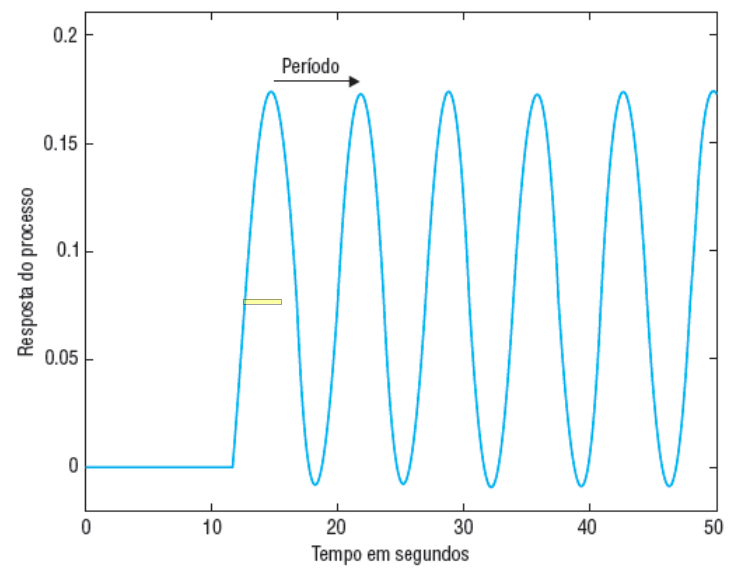
\includegraphics[width=0.4\linewidth]{Figuras/Ch14/fig3n2}
}


\frame{
	\frametitle{Exercícios}
	\begin{block}{}
		03. Dada uma entrada em degrau de $ \Delta X=3\% $, utilizando o gráfico abaixo, encontre os parâmetros de um \textbf{controlador PI}.
		
		\vspace{0.3cm}
		
		04. Dados $ K_c=3 $ e $ P_u=\SI{0.5}{\second} $, encontre os parâmetros de um \textbf{controlador PID}.
	\end{block}
	
	\centering
	\scalebox{1.2}{

\tikzset{every picture/.style={line width=0.75pt}} %set default line width to 0.75pt        

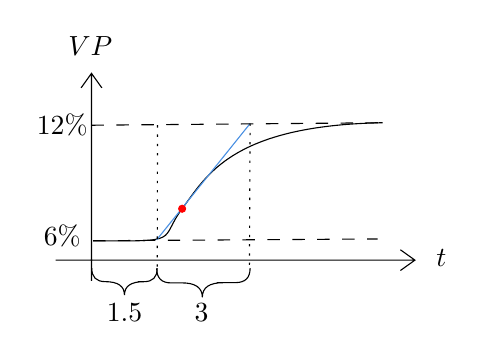
\begin{tikzpicture}[x=0.75pt,y=0.75pt,yscale=-1,xscale=1]
%uncomment if require: \path (0,300); %set diagram left start at 0, and has height of 300

%Shape: Axis 2D [id:dp8434144691544803] 
\draw  (61.27,196) -- (234.4,196)(78.58,106) -- (78.58,206) (227.4,191) -- (234.4,196) -- (227.4,201) (73.58,113) -- (78.58,106) -- (83.58,113)  ;
%Curve Lines [id:da3393494842698659] 
\draw    (79.33,186.67) .. controls (123.2,187) and (110.65,186.84) .. (122.25,171.24) .. controls (133.85,155.64) and (145.88,131.07) .. (218.8,129.8) ;


%Straight Lines [id:da773558557641419] 
\draw [color={rgb, 255:red, 74; green, 144; blue, 226 }  ,draw opacity=1 ]   (155,130.2) -- (110,186.2) ;


%Shape: Circle [id:dp28048312241562945] 
\draw  [color={rgb, 255:red, 255; green, 0; blue, 0 }  ,draw opacity=1 ][fill={rgb, 255:red, 255; green, 0; blue, 0 }  ,fill opacity=1 ] (120.58,171.24) .. controls (120.58,170.32) and (121.33,169.57) .. (122.25,169.57) .. controls (123.17,169.57) and (123.92,170.32) .. (123.92,171.24) .. controls (123.92,172.16) and (123.17,172.91) .. (122.25,172.91) .. controls (121.33,172.91) and (120.58,172.16) .. (120.58,171.24) -- cycle ;
%Straight Lines [id:da6828905031101673] 
\draw  [dash pattern={on 4.5pt off 4.5pt}]  (78.6,131) -- (218.8,129.8) ;


%Straight Lines [id:da012395283086218845] 
\draw  [dash pattern={on 4.5pt off 4.5pt}]  (79.33,186.67) -- (216.4,185.8) ;


%Shape: Brace [id:dp15969553307240192] 
\draw   (78.71,199.86) .. controls (78.7,204.19) and (80.87,206.35) .. (85.2,206.36) -- (85.2,206.36) .. controls (91.38,206.37) and (94.47,208.54) .. (94.46,212.87) .. controls (94.47,208.54) and (97.56,206.38) .. (103.75,206.39)(100.96,206.38) -- (103.75,206.39) .. controls (108.08,206.4) and (110.24,204.24) .. (110.25,199.91) ;
%Shape: Brace [id:dp058145123409859556] 
\draw   (110,200) .. controls (110.02,204.67) and (112.36,206.99) .. (117.03,206.97) -- (121.96,206.95) .. controls (128.63,206.92) and (131.97,209.23) .. (131.99,213.9) .. controls (131.97,209.23) and (135.29,206.89) .. (141.96,206.86)(138.96,206.87) -- (148.03,206.83) .. controls (152.7,206.81) and (155.02,204.47) .. (155,199.8) ;
%Straight Lines [id:da9569907625895342] 
\draw  [dash pattern={on 0.84pt off 2.51pt}]  (155,130.2) -- (154.68,198.45) ;


%Straight Lines [id:da25982411660347404] 
\draw  [dash pattern={on 0.84pt off 2.51pt}]  (110.4,131) -- (110.25,200.52) ;



% Text Node
\draw (247.2,194.8) node   {$t$};
% Text Node
\draw (78,93) node   {$VP$};
% Text Node
\draw (94.53,221.43) node   {$\SI{1.5}{\second}$};
% Text Node
\draw (131.58,221.2) node   {$\SI{3}{\second}$};
% Text Node
\draw (64.5,131) node   {$12\%$};
% Text Node
\draw (64.5,184.5) node   {$6\%$};


\end{tikzpicture}
}
}


\section*{Referências}
\frame{
	\frametitle{Referências e Exercícios Complementares}
	\begin{itemize}
		\item BAYER, Fernando Mariano; ARAÚJO, Olinto César Bassi de. Controle Automático de Processos, 3 ed. UFSM : Colégio Técnico Industrial de Santa Maria, 2011.
	\end{itemize}
	%\centering{\alert{Página 546 - \textbf{Capítulo 6}}} \\
	%\centering{\alert{Lista de exercícios 01}}
}